\begin{tcolorbox}[colback=blue!5!white,colframe=blue!75!black,title=I2C]
	Es un puerto y protocolo de comunicación serial, define la trama de datos y las conexiones físicas para transferir bits entre 2 dispositivos digitales. El puerto incluye dos cables de comunicación, SDA (Datos seriales) y SCL (reloj serial). Además el protocolo permite conectar hasta 127 dispositivos esclavos con esas dos líneas, con hasta velocidades de 100, 400 y 1000 kbits/s. \end{tcolorbox}

\begin{tcolorbox}[colback=blue!5!white,colframe=blue!75!black,title=Arduino] El\textbf{ Arduino Uno} es una placa de microcontrolador de código abierto basado en el microchip \textbf{Atmega328P} y desarrollado por \textbf{Arduino}. La placa está equipada con conjuntos de pines de E/S digitales y analógicas que pueden conectarse a varias placas de expansión y otros circuitos.
   \end{tcolorbox}

	

Para la elección del microcontrolador se analizó varios dispositivos, como por ejemplo \textbf{Arduino MEGA}, \textbf{Arduino NANO}, \textbf{EDUCIAA}, entre otros. Se llegó a la conclusión que Arduino UNO era un microcontrolador de bajo costo, baja complejidad en la programación, con librerías de diversos sensores y que cumplía con las prestaciones necesarias (señal de PWM, comunicación \textbf{I2C}, entradas analógicas y digitales).


Para comenzar con las pruebas, lo primero que se realizó es la conexión de diversos sensores en una protoboard. Se obtuvieron datos para elegir cuál  convenía utilizar, ya que se hicieron pruebas con varios sensores de temperatura, humedad y presión atmosférica.


Cabe destacar que para la comunicación de estos sensores se utilizó \textbf{comunicación I2C}, que permitió, a través de dos líneas de comunicación, conectar, en una primera instancia,  5 elementos al mismo bus.


Como paso siguiente se eligieron los sensores. Los elementos que se decidió utilizar generaban menor variación y menor error en comparación con el instrumento \textbf{TESTO 435} y estos fueron los siguientes:

\begin{itemize}
	\item  \textbf{BME280:} Sensor de presión atmosférica, temperatura y humedad relativa.
	\item \textbf{SI7021:} Sensor de temperatura y humedad relativa.
	\item \textbf{MPXV7002:} Sensor de presión diferencial.
	\item \textbf{ADS1115:} Convertidor analógico digital 16bits.
\end{itemize}

Una vez que se tuvo seguridad con los sensores elegidos se procedió a realizar una placa con estos elementos para que no se desconecten y no se produzcan errores como solía suceder mientras estaban en la protoboard. \\
\begin{figure}[htb]
	\centering
	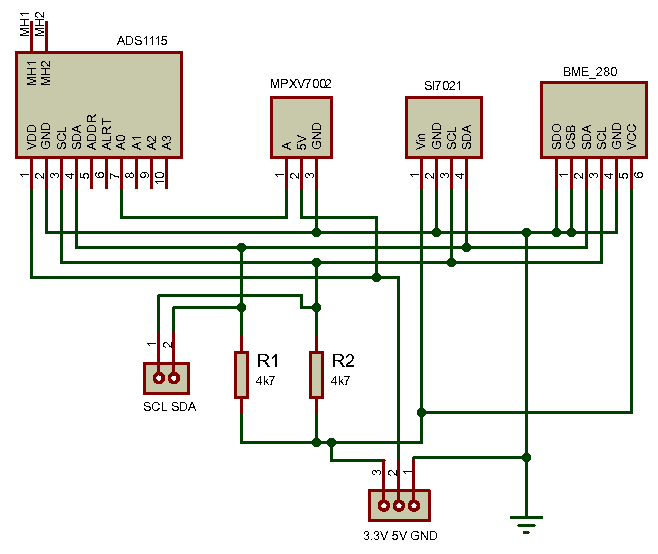
\includegraphics[scale=0.8]{placa_sensores.pdf}
	\captionof{figure}{Placa con sensores}
	\label{fig:sensoresa}
\end{figure}

A raíz de varias mediciones, durante distintos días, y realizando el contraste con el instrumento \textbf{TESTO 435} se decidió sacar de la caja donde estaban a los sensores de Temperatura y humedad para que luego el cálculo de la velocidad del aire no esté desfasado, ya que esta caja utilizada generaba un ambiente distinto al real dentro del laboratorio. \hl{ver si se agrega esto}

Estas mismas pruebas sirvieron para probar y corroborar el funcionamiento del \textbf{MPXV7002}, un sensor de diferencia de presión de alto costo en el país. Este sensor es capaz de medir de -2kPa a 2kPa en un rango de 4V (0.5 a 4.5V), para este proyecto se utilizó la parte positiva de los valores por lo que la resolución estaba establecida por los 2V de rango y 2kPa. Estos datos se ingresaron al programa \textbf{Arduino} a través de un conversor \textbf{ADS 1115} con comunicación I2C.

No se utilizó el ADC interno del microcontrolador Arduino Uno ya que es de 10 bits y el externo de 15 bits más un bit de signo, este mismo posee un amplificador de ganancia programable (PGA) que establece la escala completa, es decir, indica el valor de referencia. En Arduino este valor viene determinado por el voltaje de referencia que en el caso de Arduino UNO es 5V. En el ADS1115 lo establece el PGA. Por defecto este valor de referencia es ±6,144 V, quiere decir que el valor de 32.677 (valor máximo con 15-bit) corresponde a 6,144 V.

Ejemplo Factor de escala de Arduino UNO:
\begin{center}
	\begin{math}Factor\;de\;escala=\frac{5\;V}{1023}=\;0,0048875\;V\;=\;4,88\;mV
	\end{math}
\end{center}
Ejemplo Factor de escala de ADS115:
\begin{center}
	\begin{math}Factor\;de\;escala=\;\frac{6.144\;V}{32677}=\;0,0001875\;V\;=\;0,1875\;mV
	\end{math}
\end{center}

En la siguiente tabla se tiene un resumen de los valores posibles de factor de escala para ADS1115.
\begin{table}[h]
	\centering
	\begin{tabular}{|c|c|c|}
		\hline
		\textbf{PGA} & \textbf{Referencia (V)} & \textbf{Factor de Escala (mV)} \\ \hline
		2/3          & 6,144                   & 0,1875                         \\ \hline
		1            & 4,096                   & 0,125                          \\ \hline
		4            & 1,024                   & 0,0312                         \\ \hline
		8            & 0,512                   & 0,0156                         \\ \hline
		16           & 0,256                   & 0,0078                         \\ \hline
	\end{tabular}
\end{table}

Aunque la mayor referencia sea de 6,1444 V, el ADS1115 sólo puede medir el valor de alimentación (VDD) más 0,3 V por sus pines analógicos. \hl{ver porq} pin ingresa la señal en proteus. Por lo tanto, si alimentamos el ADS1115 con 5V, sólo podremos medir tensiones por los pines analógicos hasta 5V + 0,3V es decir, 5,3V. Lo mismo ocurriría si alimentamos con 3,3V. En este caso el máximo sería 3,6V. \hl{(con que} alimentamos? ver en proteus)\\
En el caso de este proyecto, se utilizó un valor de PGA de 1, tomando como voltaje de referencia 4,096V.
\begin{center}
	\begin{math}
		Factor\;de\;escala=\;\frac{4,096\;V}{32677}=\;0,000125\;V\;=\;0,125\;mV
	\end{math}
\end{center}

\subsection{Ecuación velocidad del aire}
El Laboratorio de Mecánica de Fluidos, antes de comenzar con este proyecto utilizaba un archivo Excel para hacer la corrección de la velocidad del aire. En este se calcula matemáticamente la densidad del aire en función de la presión, temperatura y humedad atmosférica.
%	densidad_funcion_P_T_H.pdf  dentro del drive
\begin{align}
	\rho&=\frac{3,48353\;10^{-3}\;kg\;K\;J^{-1}\;\cdot p\cdot\;(1-0,378\;\cdot\;x_v)}{Z\;\cdot\;T} \label{ec_den}\\
	x_v&=\frac{(\alpha+\beta\cdot p+\gamma\cdot t^2)\cdot(1Pa\cdot\;e^{AT^2+BT+C+D/T)})\cdot h/100}p\\
	Z&=\;1-\frac pT\cdot\lbrack a_0+a_1t+a_0t^2+(b_0+b_1t)x_v+(c_0+c_1t)x_v^2\rbrack+(d+x_v^2)\frac{p^2}{T^2}
\end{align}
\\
dónde:\\
- \textbf{p } [Pa] es la presión atmosférica medida,\\
- \textbf{t } [$^{\circ}$C] es la temperatura medida,\\
- \textbf{T } [K] es la temperatura absoluta (\textbf{T}=\textbf{t} + 273,15 \textbf{K})\\
- \textbf{h } [\%] es la humedad relativa medida,\\
- y las constantes \textbf{A,B,C,D,} $\boldsymbol{\alpha , \beta  , \gamma , a_0, a_1 ,a_2 ,b_0  ,b_1 , c_0 , c_1, D. }$


Finalmente, la ecuación anteriormente nombrada es utilizada para el cálculo final de la velocidad del aire dentro del mismo archivo.
\begin{equation}
	\triangle P=\frac{v^2\rho}2\rightarrow\;\;v=\sqrt{\frac{2\;.\;\triangle P\;}\rho}
	\label{ec_aire}
\end{equation}

Tanto las ecuaciones de densidad (\ref{ec_den})
 y la ecuación del cálculo de velocidad  (\ref{ec_aire})
  se desarrolló dentro del programa de \textbf{Arduino} para observar como dato final la velocidad del aire.


\subsection{Filtros}
\begin{tcolorbox}[colback=blue!5!white,colframe=blue!75!black,title=Mediana]
	Es una técnica de filtrado digital no lineal que suele utilizarse para eliminar el ruido de una imagen o señal. La mediana es el número que está justo en el medio de un conjunto de datos ordenados de menor a mayor o de mayor a menor.
	La idea principal del filtro de mediana es recorrer la señal entrada, sustituyendo cada dato por la mediana de una ventana de “N” datos.
\end{tcolorbox}

Una vez que se procedió a tomar diversos valores, se notó necesario la implementación de un filtro. Para esto se utilizaron varias librerías de \textbf{Arduino} para generar distintas pruebas (Figura \ref{fig:filtros}).

\begin{figure}[!h]
	\centering
	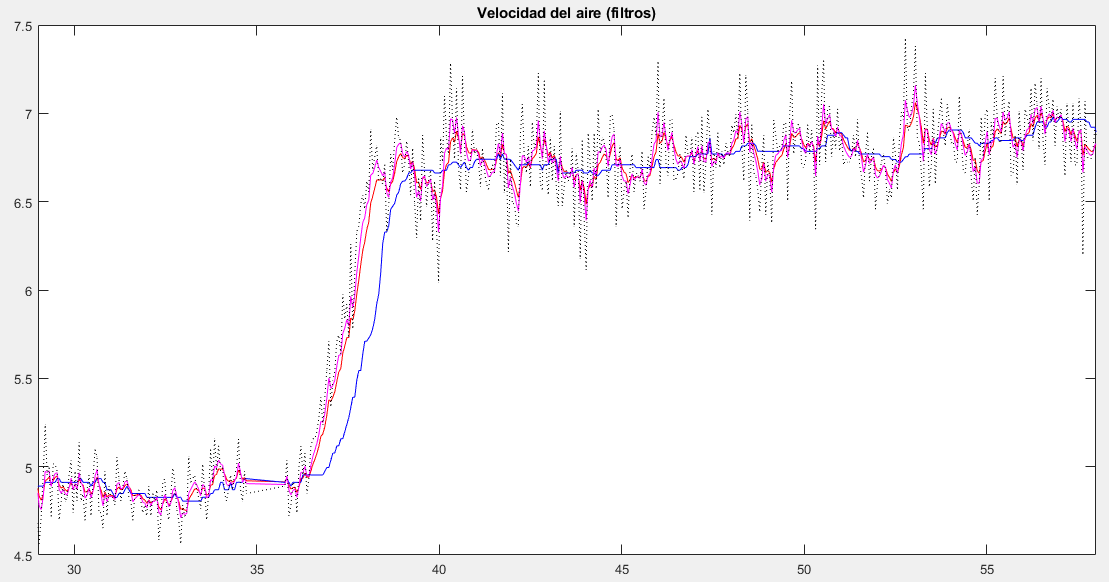
\includegraphics[scale=0.35]{filtros.png}
	\captionof{figure}{Datos y diversos filtros}
	\label{fig:filtros}
\end{figure}

Luego de varias pruebas, se eligió un filtro de mediana (Figura \ref{fig:filtrosm}) con una ventana 40, que producía menor ruido en la velocidad del aire. Se implementó en el programa de \textbf{Arduino} utilizando la una función preestablecida.

\begin{figure}[htb]
	\centering
	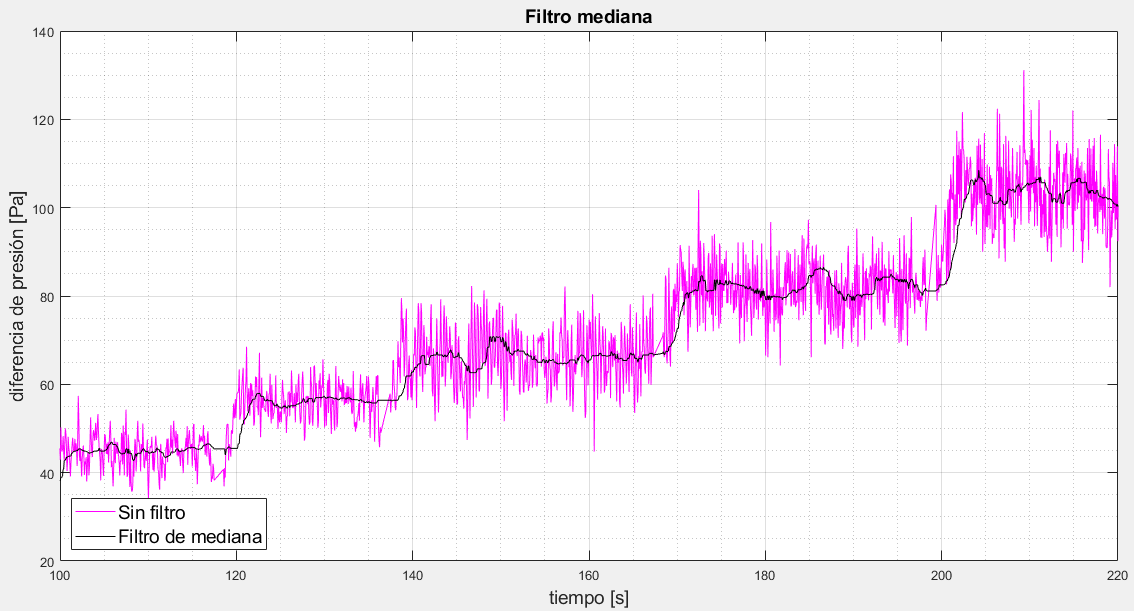
\includegraphics[scale=0.35]{filtro mediana.png}
	\captionof{figure}{Datos y filtro mediana}
	\label{fig:filtrosm}
\end{figure}


\subsection{Error observado}
Las pruebas anteriores eran realizadas con el uso normal que se le daba al variador de velocidad utilizando el panel digital frontal.

Luego, para comenzar con las pruebas de otros modos de funcionamiento del variador, se utilizó el potenciómetro frontal. Al utilizar este modo se originó error en la aceleración.   Al hacer las averiguaciones pertinentes, esto se debió a una configuración interna del variador: si se utiliza con el panel digital frontal, la curva de aceleración y desaceleración sigue una “s”, no realizando un cambio brusco en la velocidad del motor, en cambio, para el uso del potenciómetro u otro modo de funcionamiento la curva es lineal . Para revertir esto, se modificó el tiempo de aceleración y desaceleración a 20 segundos.

\begin{figure}[htbp]
	\centering
	\subfigure[Tipo s]{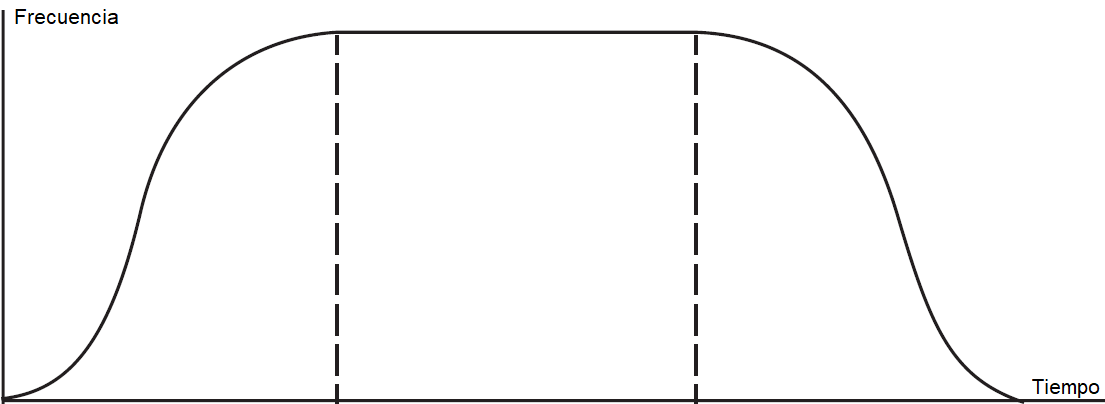
\includegraphics[width=60mm]{conS.png}}
	\subfigure[Tipo lineal]{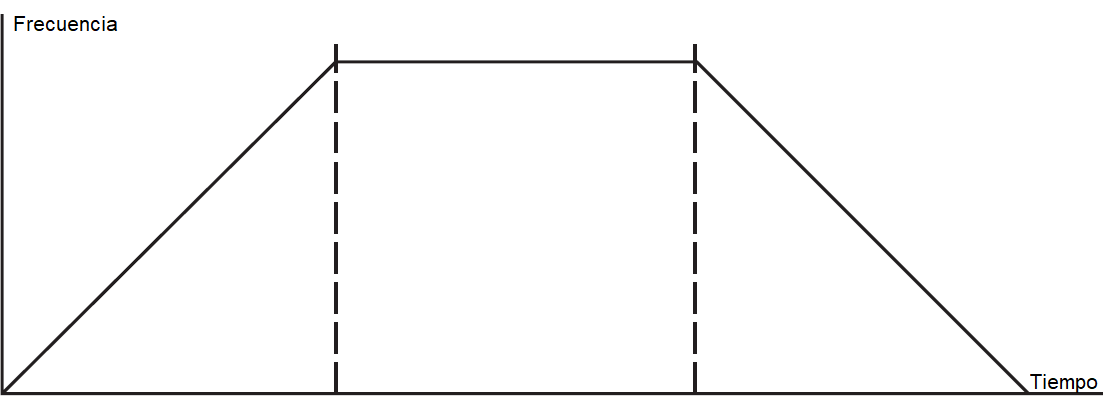
\includegraphics[width=60mm]{sinS.png}}
	\caption{Curva aceleración y desaceleración} \label{fig:curva}
\end{figure}

\newpage